\documentclass{ifacconf}

\usepackage{graphicx}
\usepackage{natbib} 

\usepackage{amsmath}
\DeclareMathOperator{\dd}{\mathrm{d}}
\DeclareMathOperator*{\argmax}{arg\,max}
\DeclareMathOperator{\lt}{lt}
\usepackage{bm}
\usepackage{nicefrac} 

\usepackage{xcolor}

\usepackage{tikz}
\usetikzlibrary{trees,positioning}

\usepackage{url}
\begin{document}
\begin{frontmatter}

\title{Bayesian Inference for Missing Physics} 

\author[First,Second,Third]{Arno Strouwen} 

\address[First]{Strouwen Statistics (e-mail: contact@arnostrouwen.com)}
\address[Second]{Biosystems Department, 
   KULeuven, Leuven, Belgium}
\address[Third]{PumasAI maybe}
\begin{abstract} % Abstract of not more than 250 words.
Model-based approaches for (bio)process systems often suffer from incomplete knowledge of the underlying physical, chemical, or biological laws.
Universal differential equations, which embed neural networks within differential equations, have emerged as powerful tools to learn this missing physics from experimental data.
However, neural networks are inherently opaque, motivating their post-processing via symbolic regression to obtain interpretable mathematical expressions.
Genetic algorithm-based symbolic regression is a popular approach for this post-processing step, but provides only point estimates and cannot quantify the confidence we should place in a discovered equation.
We address this limitation by applying Bayesian symbolic regression, which uses Reversible Jump Markov Chain Monte Carlo to sample from the posterior distribution over symbolic expression trees.
This approach naturally quantifies uncertainty in the recovered model structure.
We demonstrate the methodology on a Lotka-Volterra predator-prey system and a fed-batch bioreactor case study ...
\end{abstract}

\begin{keyword}
Bayesian inference, missing physics, symbolic regression, universal differential equations, model selection, neural network, Reversible Jump Markov Chain Monte Carlo
\end{keyword}

\end{frontmatter}

\section{Introduction}
Model-based approaches are fundamental to the analysis, control, and optimization of (bio)process systems.
These models encode knowledge of physical, chemical, and biological laws, such as conservation laws, transport phenomena, and reaction kinetics.
Such knowledge is typically expressed as systems of nonlinear differential equations.

In practice, however, our knowledge of the governing laws is often incomplete.
These knowledge gaps are termed missing physics and must be inferred from experimental data \citep{harlim}.

Universal Differential Equations (UDEs) have recently emerged as a powerful framework for learning missing model structure \citep{rackauckas1}.
UDEs embed neural networks within differential equation systems to represent terms whose underlying form is unknown \citep{dandekar}.

The opaque nature of neural networks is often undesirable in scientific computing, where interpretability and physical insight are valued.
Consequently, UDE-based approaches are frequently combined with interpretable machine learning techniques, such as sparse regression \citep{kaiser} or symbolic regression \citep{koza}.
These techniques distill the neural network into human-understandable mathematical expressions.

Symbolic regression searches the space of mathematical expressions to find models that balance accuracy and simplicity.
Mathematical expressions are typically represented as tree data structures, where internal nodes correspond to operators and leaf nodes to variables or constants.

UDE-based methods are rapidly gaining traction across scientific domains, including physics \citep{keithLearningOrbitalDynamics2021}, chemistry \citep{santanaEfficientHybridModeling2023}, and biology \citep{philippsNonNegativeUniversalDifferential2024, rojas-camposLearningCOVID19Regional2023}.

When symbolic regression is employed in these applications, genetic algorithms are the dominant approach for exploring the space of candidate expression trees \citep{cranmer}.
While genetic algorithms often yield good point estimates for the missing physics, they provide no principled way to quantify uncertainty in the discovered model structure.

Recently, symbolic regression has been formulated within a Bayesian framework \citep{jin}.
This approach replaces genetic algorithms with Reversible Jump Markov Chain Monte Carlo (RJMCMC) to explore the space of possible model structures.
RJMCMC extends standard MCMC by allowing moves between parameter spaces of different dimensions.
This capability is essential for symbolic regression because different expression trees contain different numbers of constant parameters.
The likelihood of a candidate tree is evaluated by comparing its predictions to the outputs of the trained neural network.
A prior distribution over trees that penalizes depth encourages parsimonious expressions, embodying Occam's razor.
The RJMCMC sampler generates samples from the posterior distribution over symbolic trees, naturally quantifying structural uncertainty.
In this paper, we apply Bayesian symbolic regression to the missing physics problem.

LV, Bioreactor
\section{Motivating example: Lotka-Volterra}
\begin{equation}\label{eq:lv}
\begin{aligned}
\frac{dx}{dt} &= \alpha x - \beta xy,\\
\frac{dy}{dt} &= -\gamma y + \delta xy,\\
\end{aligned}
\end{equation}
missing
\begin{equation}\label{eq:lv-missing}
\begin{aligned}
\frac{dx}{dt} &= \alpha x - \mathord{?}\\
\frac{dy}{dt} &= -\gamma y + \mathord{?},\\
\end{aligned}
\end{equation}
\section{Universal differential equation}
We consider dynamical systems of the following form:
\begin{equation}\label{eq:system}
\begin{aligned}
	\frac{\dd \bm x}{\dd t} &= \bm f(t,\bm x,\bm \phi(\bm g(\bm x))), \qquad \text{with } \bm x(t=0) = \bm x_0;\\
	\bm y_k &= \bm h(\bm x(t_k)) + \bm \epsilon_k,
\end{aligned}
\end{equation}
where $t$ denotes time and $\bm x(t)$ is the state vector.
The states evolve according to the ordinary differential equation system $\bm f$ with initial conditions $\bm x_0$.
Measurements $\bm y_k$ are collected at discrete time points $t_k$ and are related to the states through the observation function $\bm h$.
This function is useful for example when only a subset of states is observed.
The measurements are corrupted by independent Gaussian noise $\bm \epsilon_k$, with each $\bm \epsilon_k$ identically and independently distributed as multivariate normal with zero mean and covariance matrix $R$.

The system $\bm f$ depends on the unknown function $\bm \phi$, which represents the missing physics.
The input to $\bm \phi$ is the output of a known preprocessing function $\bm g(\bm x)$.
This function $\bm g$ is useful when the missing physics depends only on a subset of the states or on known transformations thereof.
We refer to $\bm g(\bm x)$ as the features.

In the UDE framework, the unknown function $\bm \phi$ is replaced by a neural network:
\begin{equation}\label{eq:UDE}
	\frac{\dd \bm x}{\dd t} = \bm f(t,\bm x,\text{NN}(\bm g(\bm x), \bm \theta)).
\end{equation}
The neural network $\text{NN}(\bm g(\bm x), \bm \theta)$ takes the features $\bm g(\bm x)$ as input and depends on parameters $\bm \theta$ that must be learned from experimental data.
Training of $\bm \theta$ proceeds by minimizing the log-likelihood of the observations.

applied to LV
 
\section{Bayesian symbolic regression}
We want to find mathematical expressions which match the output of the neural network and quantify how certain we are a specific expression is correct.
Mathematical expressions can be represented by a tree data structure.
The non-terminal nodes of the tree contain mathematical operators,
while the terminal nodes contain either features or constants.
Each operator node has one or two children, depending on its order, i.e. if it is a unary or binary mathematical operator.
All terminal nodes contain features except a special linear transformation operator $\lt(x,a,b)=ax+b$, here the second and third child, $a$, and $b$ are constants, and the first child $x$ is either an operator or a feature.
This $\lt$ operator is the only way for constants to enter the mathematical expression.
Figure~\ref{fig:tree} illustrates this tree representation.

\begin{figure}[htbp]
\centering
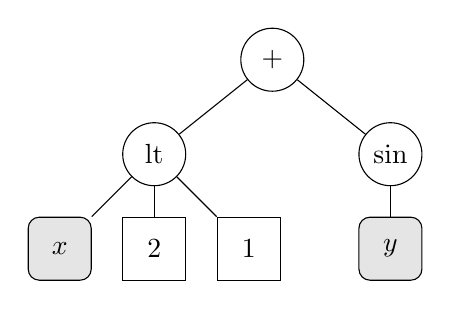
\begin{tikzpicture}[
    level distance=1.2cm,
    sibling distance=2.5cm,
    every node/.style={draw, circle, minimum size=8mm, inner sep=1pt},
    edge from parent/.style={draw, -},
    level 1/.style={sibling distance=3cm},
    level 2/.style={sibling distance=1.2cm},
    feature/.style={draw, rectangle, rounded corners, fill=gray!20},
    const/.style={draw, rectangle, fill=white}
]
\node {$+$}
    child {node {$\lt$}
        child {node[feature] {$x$}}
        child {node[const] {$2$}}
        child {node[const] {$1$}}
    }
    child {node {$\sin$}
        child {node[feature] {$y$}}
    };
\end{tikzpicture}
\caption{Expression tree representing $2x + \sin(y)$. Circular nodes contain operators ($+$, $lt$, $\sin$). Rectangular nodes are terminals: rounded rectangles denote features ($x$, $y$), and plain rectangles denote constants. The $lt$ node implements the linear transformation $\lt(x,2,1) = 2x + 1$.}
\label{fig:tree}
\end{figure}

To perform Bayesian inference, we must specify a prior distribution over trees and a likelihood function.
\subsection{Prior}
The prior over trees is constructed from several component distributions.
The \textit{terminal prior} specifies the probability that a node at a given depth is a leaf node.
This probability increases with depth to discourage overly complex trees.
The \textit{feature prior} assigns probabilities to different features at leaf nodes.
The \textit{operator prior} assigns probabilities to different operators at branch nodes.
Finally, \textit{priors for $a$ and $b$} specify distributions over the constants in $\lt$ nodes.

Using these distributions, the prior over trees is defined recursively.
Starting at the root (depth zero), the terminal prior determines whether the node is a leaf or branch node.
If the node is a leaf, a feature is sampled from the feature prior.
If the node is a branch, an operator is sampled from the operator prior.
If this operator is $\lt$, then constants $a$ and $b$ are also sampled from their respective priors.
Child nodes are then generated recursively with incremented depth.

Sampling a tree from the prior thus involves both discrete choices (whether nodes are leaves or branches, selection of features and operators) and continuous choices (the constants $a$ and $b$ in $\lt$ nodes).
We denote the collection of discrete choices by $T$ and the continuous choices by $A$ and $B$, which contain the $a$ and $b$ constants in depth-first order.
Note that the dimensions of $A$ and $B$ vary across trees, as different trees contain different numbers of $\lt$ nodes.

The tree will not fit the neural network output exactly.
We assume the discrepancy follows an additive i.i.d. normal distribution with variance $\sigma^2$.
A \textit{variance prior} on $\sigma$ completes the Bayesian specification.

We use the notation $p(T, A, B, \sigma)$ to denote the prior density for a given tree.
\subsection{Likelihood}
Let $T(\bm g(\bm x_k), A, B)$ denote the output of a tree evaluated at the features $\bm g(\bm x_k)$ with constants $A$ and $B$.
Since each tree produces a scalar output, a neural network with $m$ outputs requires $m$ separate trees $T_1, \ldots, T_m$, each with its own structure and constants $(T_j, A_j, B_j)$.
We denote the $j$-th output of the neural network as $\text{NN}_j(\bm g(\bm x_k), \bm \theta)$.

The log-likelihood for output $j$ at time point $k$ is:
\begin{equation}\label{eq:likelihood}
\begin{aligned}
    &\log p(\text{NN}_j(\bm g(\bm x_k), \bm \theta) | T_j, A_j, B_j, \sigma_j) =\\
    &\quad -\frac{1}{2}\log(2\pi\sigma_j^2) -\frac{\left( T_j(\bm g(\bm x_k), A_j, B_j) - \text{NN}_j(\bm g(\bm x_k), \bm \theta) \right)^2}{2\sigma_j^2}.
\end{aligned}
\end{equation}
Assuming independence across time points and outputs, the total log-likelihood is the sum over all $k$ and $j$.
For notational simplicity, we write this as $p(\text{NN}_j | \{T_j, A_j, B_j, \sigma_j\})$, with analogous notation for the posterior.
\subsection{Markov-Chain}
Since the trees for different neural network outputs are independent, we run a separate Markov chain for each output $j$.
In the following, we describe the sampler for a single tree, dropping the subscript $j$ for clarity.

We use hybrid Gibbs sampling \citep{tierney} with two transition kernels.
The first kernel updates only the continuous parameters $\sigma$, $A$, and $B$, holding the tree structure $T$ fixed.
Since these parameters are continuous, we can use efficient gradient-based samplers such as NUTS \citep{hoffman}.

The second kernel updates the discrete tree structure $T$ using Reversible Jump Markov Chain Monte Carlo (RJMCMC) \citep{green}.
RJMCMC proposes random modifications to the tree structure.
Modifications that increase the posterior probability are always accepted, while those that decrease it are accepted with a probability that maintains detailed balance.
This ensures the stationary distribution of the Markov chain is the posterior distribution.

Changing the tree structure cannot be done independently of the continuous parameters, since $\lt$ nodes may appear or disappear.
This change in dimensionality of $A$ and $B$ requires careful treatment in RJMCMC.


Let $K(T^*, A^*, B^* | T, A, B)$ denote the transition kernel, which defines a probability distribution over the next state $(T^*, A^*, B^*)$ given the current state $(T, A, B)$.

We only consider modifications where $\lt$ nodes are either added or deleted, but not both simultaneously.
When $\lt$ nodes are added, the new constants $a$ and $b$ are sampled from their respective priors.
We denote these newly sampled parameters as $u_A$ and $u_B$.

To maintain the detailed balance, we require that:
\begin{equation}\label{eq:balance}
\begin{aligned}
p(T, A, B, \sigma|\text{NN})
K(T^*, A^*, B^* | T, A, B)dA^*dB^*=\\
p(T^*, A^*, B^* |, \sigma\text{NN})
K(T, A, B | T^*, A^*, B^*)dAdu_AdBdu_B
\end{aligned}
\end{equation}
If a bijection $\psi$ can be established between
$(A, u_A, B, u_B)$ and $(A^*, B^*)$,
then we get:
\begin{equation}\label{eq:substitute}
dA^*dB^*=\\
\left | \det \frac{\partial \psi}{\partial A \partial u_A \partial B  \partial u_B } \right |
dAdu_AdBdu_B
\end{equation}
Such a bijection is straightforward to construct: $A^*$ is formed by inserting $u_A$ at positions corresponding to new $\lt$ nodes in depth-first order, and similarly for $B^*$.
Since this is a permutation, the absolute value of the determinant is $1$, and thus:
\begin{equation}\label{eq:balance_simpliflied}
\begin{aligned}
K(T^*, A^*, B^* | T, A, B) = \\
K(T, A, B | T^*, A^*, B^*)\frac{p(T^*, A^*, B^* |, \sigma\text{NN})}{p(T, A, B, \sigma|\text{NN})}
\end{aligned}
\end{equation}

The same argument applies when $\lt$ nodes are deleted: the removed parameters $u_A$ and $u_B$ can be extracted from $A$ and $B$ via the inverse permutation, and (\ref{eq:balance_simpliflied}) still holds.

We split the transition kernel into two factors:
$q(T^*, A^*, B^* | T, A, B)$ denotes the proposal distribution for modifying the tree $(T, A, B)$ into $(T^*, A^*, B^*)$,
and $\alpha(T^*, A^*, B^*, \sigma | T, A, B, \sigma)$ denotes the acceptance probability.
If the proposal is rejected, the tree remains unchanged for this iteration.

By setting:
\begin{equation}
\begin{aligned}
\log \alpha(T^*, A^*, B^* | T, A, B) = \\
\min ( 0, \log p(T^*, A^*, B^*, \sigma|\text{NN}) -  \log p(T, A, B, \sigma|\text{NN})\\
 \log q(T, A, B | T^* A^*, B^*) -  \log q(T^*, A^*, B^* | T, A, B)),
\end{aligned}
\end{equation}
equation (\ref{eq:balance_simpliflied}) is always satisfied.
In practice, we sample $u \sim \text{Uniform}(0,1)$ and accept the proposal if $\log u < \log \alpha$.
Note that this derivation mirrors standard random walk Metropolis-Hastings, but with special care for the transdimensional nature of the problem: the bijection $\psi$ accounts for parameters appearing or disappearing when $\lt$ nodes are added or removed.

The proposal distribution $q$ follows \citet{jin} and consists of several move types:

With probability $p_{rf}$, the tree \textbf{reassigns a feature}: a randomly selected leaf node is replaced with a feature sampled from the feature prior.
The reverse move reassigns the old feature to the same node.
Since no $\lt$ nodes change, the acceptance ratio simplifies to:
\begin{equation}
\begin{aligned}\label{eq:reasign}
\log R &= \log p(\text{NN}|T^*, A, B, \sigma) - \log p(\text{NN}|T, A, B, \sigma)
\\ &+ \log p(T^*, A, B, \sigma) - \log p(T, A, B, \sigma).
\end{aligned}
\end{equation}
The proposal probabilities cancel because the forward and reverse moves occur with equal probability.
With a uniform feature prior, this further simplifies to only the likelihood ratio.

With probability $p_{ro}$, the tree \textbf{reassigns an operator}: a randomly selected branch node is replaced with an operator of the same arity.
If no branch node exists, the tree is unchanged.
The acceptance ratio is the same as (\ref{eq:reasign}).

With probability $p_p$, the tree is \textbf{pruned}: a randomly selected branch node is replaced by a leaf node drawn from the feature prior.
If no branch nodes exist, the tree is unchanged.
The reverse of pruning is growing.

With probability $p_g$, the tree is \textbf{grown}: a randomly selected leaf node is replaced by a subtree sampled from the prior, conditioned on the node's depth.
To ensure grow is the reverse of prune, the root of the new subtree must be a branch node; if a leaf is sampled, it is resampled until a branch node is obtained.

With prob the tree is deleted

With pro the tree is expanded

Of course, probabilities add to one.
\section{Computational Details}
\section{Bioreactor Case Study}
We illustrate the concept of missing physics with a well-mixed fed-batch bioreactor example. This reactor has a long history in the MbDoE literature \citep{versyck, telen, telen2, houska}.
the substrate concentration, $C_s$,
the biomass concentration, $C_x$,
and the volume of the reactor, $V$.
The evolution in time of these states is governed by the following differential equations:
\begin{equation}\label{eq:bioreactor}
\begin{aligned}
\frac{dC_s}{dt} &= -\left(\frac{\mu(C_s)}{y_{x,s}} + m\right) C_x + \frac{Q_{in}(t)}{V}(C_{S,in} - C_s),\\
\frac{dC_x}{dt} &= \mu(C_s) C_x - \frac{Q_{in}(t)}{V}C_x,\\
\frac{dV}{dt} &= Q_{in}(t).
\end{aligned}
\end{equation}
In these equations, the specific growth rate, $\mu$, is an unknown function.
This function has a single input, $C_s$.
This unknown function must be determined from experimental data.
The true function that must be recovered is the Monod equation:
\begin{equation}
\mu(C_s) = \frac{\mu_{max}C_s}{K_s + C_s}.
\end{equation}
Other example Haldane:
\begin{equation}
\mu(C_s) = \frac{\mu_{max}C_s}{K_s + C_s + \frac{C_s^2}{K_I}}.
\end{equation}


\section{Discussion}
At the start of this research project, we aimed to eliminate the neural network as an intermediate step and directly compute the likelihood based on the measured observations using (\ref{eq:system}), rather than the neural network output as in (\ref{eq:likelihood}).
However, this proved computationally infeasible: evaluating symbolic trees within a differential equation solver introduces significant overhead that cannot easily be parallelized.
Recent advances in MCMC methods for discrete parameters may make this direct approach feasible in the future.

Removing the neural network intermediate would bring additional benefits.
Models often contain unknown parameters that must be calibrated alongside the missing physics.
A likelihood based directly on (\ref{eq:system}) would enable joint uncertainty quantification over both the model structure and these parameters, yielding a fully Bayesian treatment.

This would also open the door to Bayesian experimental design for missing physics problems, an area that remains understudied.
Classical T-optimal designs \citep{strouwen} target model discrimination but are difficult to combine with designs for parameter precision.
The Bayesian framework naturally unifies these objectives \citep{chaloner}.

In summary, we have presented a Bayesian approach to symbolic regression for missing physics that provides principled uncertainty quantification over discovered model structures.
While the current two-stage approach---first training a neural network, then fitting symbolic expressions---is computationally practical, future work will focus on eliminating this intermediate step to enable fully integrated Bayesian inference and experimental design.
\bibliography{ifacconf}
\end{document}
